\chapter{Background knowledge}
\label{ch:ForNot}

This chapter will provide the reader with clear definitions of the task of entity linking as well as the basic technologies, concepts, and terminologies that are associated with the scope of this work.

\section{Problems definitions}
\label{Pbdef}
Given an input document, we want to link all mentions, represented by the set $\mathcal{M}=\{m_{i}\| 0 \leq i \leq n\}$, in it, with \textit{n} being the total number of mentions in the document, to unique entities in the set $\mathcal{E}=\{e_{i} \| 0 \leq i \leq N\}$ with N being the number of all entities in a certain knowledge base. This task is usually solved in three-step (\textit{i}) detection of mentions' boundaries (the elements of set $\mathcal{M}$), (\textit{ii}) Generation of candidate entities set ($\mathcal{C}$ a subset of $\mathcal{E}$), and finally (\textit{iii}) entity disambiguation, in other words, the selection of the most plausible candidate.\cite{Sevgili2020}

In this work, we will omit the first and the last step. We will focus solely on the candidate generation. After detecting the mentions in the text. Based on embeddings similarity metrics we generate a set of candidate entities $\mathcal{C}=\{c_{ik}\| 0 \leq i \leq n, 0 \leq k \leq K\} \subset \mathcal{E}$, with K the number of candidates generated for each mention. We will try to minimize K without losing any of the system's performance.


\section{Understanding of concepts}

\subsection{Word embeddings}
Word embeddings became one of the most prominent trends in NLP\footnote{https://towardsdatascience.com/introduction-to-word-embedding-and-word2vec-652d0c2060fa}. They are vector representations of words, such that, when we map these vectors into a space, out of certain mathematical properties we can extract semantic meaning. For instance, similarity in meaning can be deduced from spatial closeness. As an example we take the representing vector for the word "\textit{man}" and the one for the word "\textit{people}", these two vectors would be closer to one another, as would be the vector for the word "\textit{window}" to that of "\textit{man}".

\subsection{Transformer model}
\label{transformer}

\begin{figure}[h]
\centering
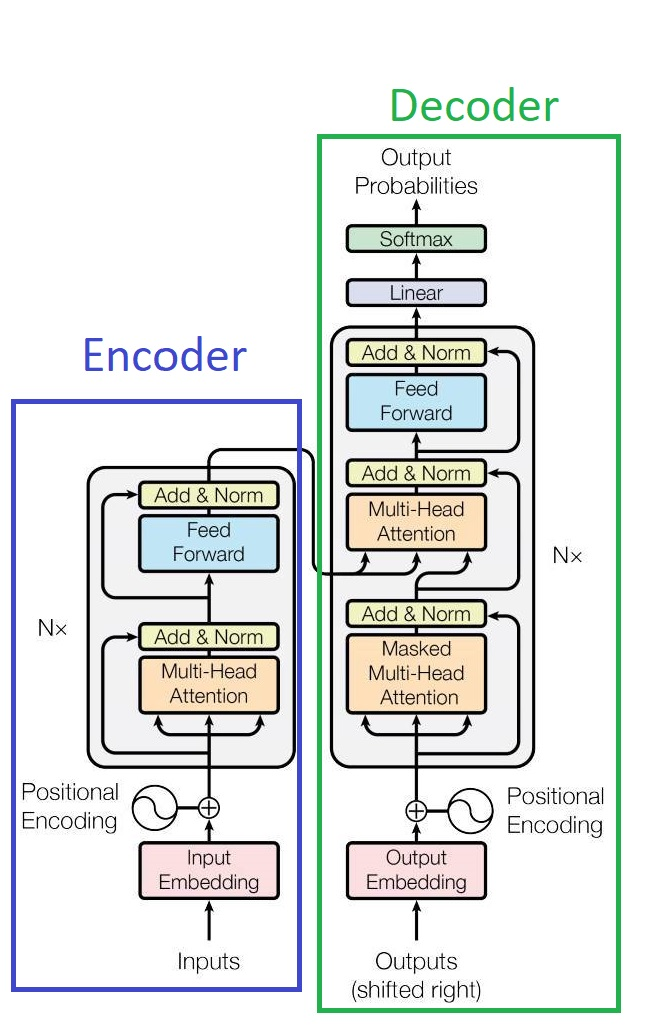
\includegraphics[width=8cm]{figures/transformer-architecture.jpg}
\caption{The transformer model architecture presented in \cite{Attention}}
\label{transformer}
\end{figure}

As mentioned previously, in our initial approach we will treat the task of candidate generation similar to a translation task. We "translate" word embeddings into entity embeddings. Using the output as the focal search point we extract the top K closest entities to our output vector, in the embedding space we translated into, as our candidates.\newline
This translation is a sequence-to-sequence mapping computed with the help of a transformer encoder block. Our implementation follows the work of \cite{Attention}, which architecture is shown in Figure \ref{transformer}. However, we do not rebuild the whole model, we just implement the encoder's block.\newline

\begin{figure}[h]
\centering
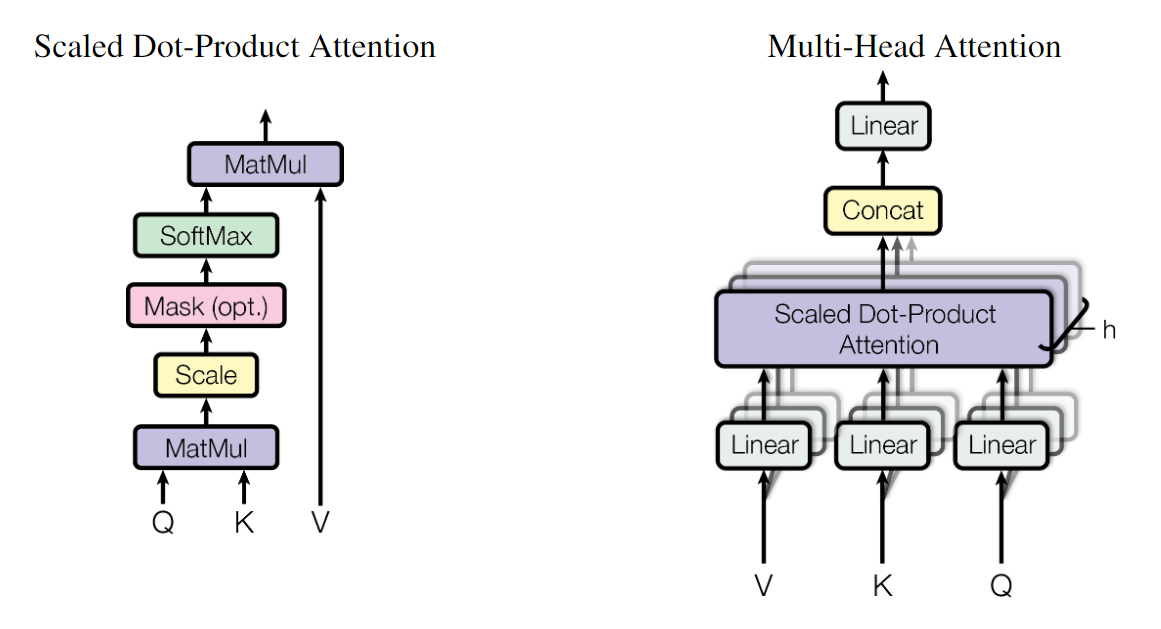
\includegraphics[width=10cm]{figures/multi-head-attention.png}
\caption{the architecture of the attention mechanism from \cite{Attention}}
\label{attention}
\centering
\end{figure}

To briefly summarize how this encoder block works, we direct our attention to Figure \ref{attention} and refer to \cite{Attention}. On the left side, we see the scaled dot product block, when mounted in parallel this provides us with a multi-head attention block. The scaled dot product attention consists of three defined matrices; $\mathcal{W}^q$, $\mathcal{W}^k$, and $\mathcal{W}^v$ (which can be optimized), respectively named; query, key, and value matrix, a scaling value, a softmax function, and an additional matrix $\mathcal{W}^o$.

Using the query and value matrix, the model computes an attention weight $a_{ij}$ for all pairs (\textit{i}, \textit{j}) in the sequence. At this stage, the scaling factor is used to scale the softmax function's input to prevent it from growing into regions with small gradients. After passing these scaled vectors to a softmax function which normalizes the weights such that $\sum_{j}^{T}a_{ij} = 1$ with T representing the length of the sequence, the model uses the output to calculate the self-attention weighted sum for each of the \textit{i}-th words in the sequence as $A_{i}= \sum_{j}^{T} a_{ij} * v_{i}$, $v_{i}$ is the \textit{i}-th row in the value matrix. These vectors are then representative of the whole context.\cite{Attention} \newline

Combining multiple of these blocks, with some additional processing forms the multi-head attention. In this case, the scaled Dot-Product attention outputs a vector of reduced dimensions, so that the concatenation of the output of h-layers sums up to the dimension of the value matrix. The latter is then multiplied by the result, giving the model the ability to attend to data from various representation subspaces at various positions.

\subsection{BERT}
To generate embeddings for the mentions in the input document, we will use a pre-trained BERT(Bi-directional Encoder Representation from Transformers)-model \cite{BERT}. BERT's architecture is based on the architecture of the bidirectional Transformer encoder presented in the previous subsection \ref{transformer}.

% There are many pre-trained BERT models. In this work, however, we implement the $BERT_{BASE}$\footnote{https://huggingface.co/bert-base-uncased}, this particular model is made out of 12 transformer blocks/layers of hidden-size equal to 768 and 12 self-attention heads, summing in total to 110M parameters.\newline

Until BERT was introduced most of its predecessors used unidirectional language models, meaning that every token can either only focus on the tokens that precede it or the tokens that succeed it in the self-attention layers. Others have tried to combine both the right-to-left and left-to-right contexts by concatenating the separately trained models, which proved to be unfruitful. \cite{BERT} \newline
BERT overcame this constraint by defining the MLM (Masked Language Modeling) pre-training objective. It consists in masking 15\% of the tokens in the input document, and then at a later stage trying to predict them. Thus they enabled the fusion of the right and left contexts. They defined a second objective as well, namely next sentence prediction that jointly pre-trains text-pair representations. In this case, the model only needs to output if the sentences are correlated or not \cite{BERT}.\newline

For the tokens it encounters, BERT employs a vocabulary of 30.000 WordPieces embeddings \cite{BERTref}  to generate vector representation on one part. These wordpieces can either be words or subwords. In this manner, they avoid the need for special treatment for unknown words and get a more effective method of dealing with rare words.\newline
On the other part, BERT employs positional embeddings. Additionally, since the BERT input can be composed of multiple sentences, a learned embedding, that denotes to which segment the token belongs to, is used.\newline
The final token's embedding is then generated by summing all these three embeddings.\newline
The resulting sequence embedding contains not only information about the individual tokens, but also information about the whole segment, which is stored in the last hidden layer of the \textit{[CLS]} token that is added to the start of each input. This vector is used in the pre-training phase for the next sentence prediction task, thus it can be easily repurposed to solve any downstream task that may require information about the whole segment \cite{BERT}.

\subsection{Knowledge Graphs}
Since 2012 and over the years, knowledge graphs have been defined in various ways\newline
\cite{ehrlinger2016towards}.\newline
In this work, we will adopt the following definition\footnote{\label{fn1}inspired from IBM's definition of KG: https://ibm.co/3CXpPuW}.\newline
Knowledge graphs are semantic networks that model real-world knowledge in the form of RDF triples i.e. (\textit{h}, \textit{p}, \textit{t}). These RDF triples can be one of two types; (\textit{i}) relational triple: where the predicate \textit{p} depicts a relation between the two entities \textit{head} entity \textit{h} and \textit{tail} entity \textit{t} or (\textit{ii}) an attribute triple: where the tail entity becomes the value of the attribute \textit{p}.
These entities and predicates are represented by nodes and edges respectively.\newline

Datasets with various structures and from various sources are usually the building blocks for Knowledge graphs. Knowledge graphs incorporate elements of many data management models\footnote{
tinyurl.com/292necwm}:
\begin{itemize}
\item{database: because organized queries may be used to explore the data;}
\item{Graphs: may be examined as any other network data structure, making them easy to investigate;}
\item{knowledge bases: Because they have formal semantics, they may be utilized to interpret data and deduce novel facts.}
\end{itemize}
\noindent Other key characteristics that knowledge graphs have are\footnote{
tinyurl.com/292necwm}:
\begin{itemize}
\item{Performance: millions of facts and properties can be efficiently managed}
\item{Expressivity: RDF(S) and OWL\footnote{https://cambridgesemantics.com/blog/semantic-university/learn-owl-rdfs/rdfs-vs-owl/}, two standards in the Semantic Web stack, enable the fluid representation of a variety of data and content kinds.}
\item{Standardization: to assure that requirements of different users are met all of the above characteristics are standardized through the W3C community\footnote{https://www.w3.org/community/};}
\end{itemize}


\subsection{Knowledge graph embeddings}
\label{kgeBK}
Similar to word embeddings a knowledge graph embedding is a vectorial representation of entities and relations of the underlying knowledge base. Research in this domain tries to keep the embedding dimension low for better performance and real-world applicability. \newline
According to a survey done \cite{KGsurvey} a Knowledge graph embedding can be characterized by four aspects;
\begin{itemize}
\item{A representation space: the space in which entities and relations are modeled.\newline In \cite{KGconditions} they define three conditions that each space should follow;\textit{(i)} differentiability, \textit{(ii)} calculation possibility, and \textit{(iii)} definability of a scoring function. Four categories of spaces are defined:}
	\begin{itemize}
	\item{Pointwise Space: The pointwise Euclidean space}
	\item{Complex Vector Space: Entities and interactions are represented in a complex space rather than a real-valued space.}
	\item{Gaussian Distribution \cite{GaussianWE}}
	\item{Manifold and Group}
	\end{itemize}
\item{A scoring function: This function will assign a plausibility score for each RDF in the representation. These commonly fall under one of the two categories;}
	\begin{itemize}
	\item{Distance-based: as an example some works \cite{TransE} rely on the addictive aspect of the embeddings, e.g. \textit{head} entity + \textit{predicate} $\approx$ \textit{tail} entity}
	\item{Semantic similarity-based: commonly implemented through the multiplicative aspect of the embedding, where \textit{head} entity's vector$\ast$ \textit{relation} matrix $\approx$ \textit{tail} entity's vector}
	\end{itemize}	
\item{Models for encoding representation and learning relational interactions. \cite{KGsurvey2} Defines two types;}
	\begin{itemize}
	\item{Triplet fact-based}
	\item{Description-based}
	\end{itemize}
\item{Embedding with auxiliary information, of which four types have been used;}
	\begin{itemize}
	\item{text descriptions}
	\item{type constraints}
	\item{relational paths}
	\item{visual information}
	\end{itemize}
\end{itemize}

The process followed by all the various knowledge graph embedding models to determine the semantic significance of the facts is essentially the same \cite{KGsurvey2}. First, initial random values are assigned to the embedding vectors of the entities and relations to learn an embedded representation of a knowledge graph. The method then constantly optimizes the embeddings starting from a training set and continuing until a stop condition is achieved. Which usually is the condition for preventing overfitting.

\subsection{Hierarchical Navigable Small Worlds Graphs}
HNSW graphs are data structures inspired by probability skip lists presented in \cite{skip-lists} and Navigable small word graphs (NSW-graph) that were presented throughout several works\newline \cite{2nd-NSW}, \cite{3rd-NSW}, and \cite{1st-NSW}.

The structure of HNSW graphs can be visualized in Figure\ref{HNSWG}. The concept of HNSWG follows along these lines; each layer is a proximity graph, a graph where nodes are connected to their nearest neighbors. The highest layer contains the longest connections and the lowest number of nodes. As we travel down the layer the number of nodes increases and the distances between them decrease \cite{HNSWG}.\newline
When querying the graph the search starts from one of the nodes in the highest layer, these are called entry points, and the route to the query vector is computed greedily. This means; starting from the entry point we travel along the edges that lead to the closest neighbor to our query vector at each step. When a local minimum is reached at a certain layer, we restart the process of finding a local minimum at the next downward layer from the local minimum that was reached. The stop condition is then finding the local minimums at the lowest layers \cite{HNSWG}.\newline

In this work the implementation of this data structure will be configured by the following three parameters;
\begin{itemize}
\item{\textit{M}, is the number of neighbors used in the graph. A larger M is more accurate but uses more memory}
\item{\textit{efSearch}, This parameter represents how many entry points will be explored between layers during the search.}
\item{\textit{efConstruction}, the number of entry points will be explored when building the index.}
\end{itemize}
A certain trade-off should be considered when setting these values, which is between the speed of the search and its efficiency. The higher the parameters are set the more accurate results the search will return and the longer it would take. Tests and results for different values of these parameters are presented in \footnote{https://www.pinecone.io/learn/faiss/}.

\begin{figure}[t!]
\centering
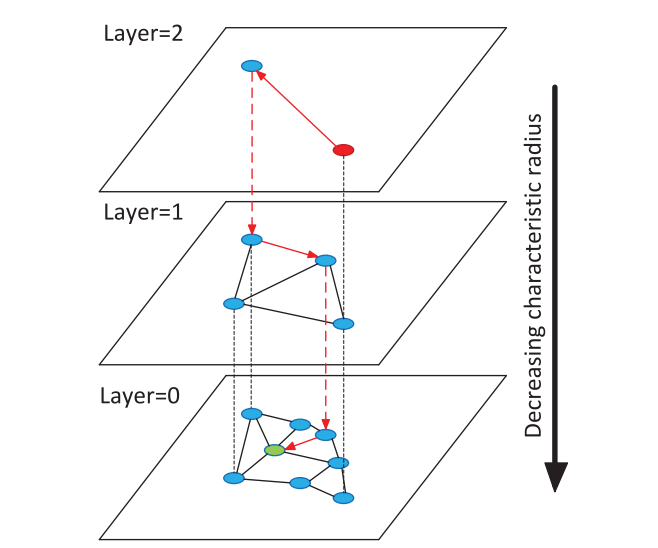
\includegraphics[width=8cm]{figures/HNSWG.png}
\caption{Structure of Hierarchical Small Worlds Graphs from \cite{HNSWG}}
\label{HNSWG}
\end{figure}

%\subsection{TransE} 
%\subsection{Attention Encoder}
%\subsection{NLP basic concepts}
%\subsection{}




